%%%%%%%%%%%%%%%%%%%%%%%%%%%%%%%%%%%%%%%%%%%%%%%%%%%%%%%%%%%%%%%%%%%%%%%%%%%%
% AGUJournalTemplate.tex: this template file is for articles formatted with LaTeX
%
% This file includes commands and instructions
% given in the order necessary to produce a final output that will
% satisfy AGU requirements, including customized APA reference formatting.
%
% You may copy this file and give it your
% article name, and enter your text.
%
%
% Step 1: Set the \documentclass
%
%

%% To submit your paper:
\documentclass[draft]{agujournal2019}
\usepackage{url} %this package should fix any errors with URLs in refs.
\usepackage{lineno}
\usepackage[inline]{trackchanges} %for better track changes. finalnew option will compile document with changes incorporated.
\usepackage{soul}
\usepackage{amsmath}
\usepackage{siunitx}
\usepackage{color}
\newcommand{\red}[1]{\textcolor{red}{#1}}
\newcommand{\blue}[1]{\textcolor{blue}{#1}}

\linenumbers
%%%%%%%
% As of 2018 we recommend use of the TrackChanges package to mark revisions.
% The trackchanges package adds five new LaTeX commands:
%
%  \note[editor]{The note}
%  \annote[editor]{Text to annotate}{The note}
%  \add[editor]{Text to add}
%  \remove[editor]{Text to remove}
%  \change[editor]{Text to remove}{Text to add}
%
% complete documentation is here: http://trackchanges.sourceforge.net/
%%%%%%%

\draftfalse

%% Enter journal name below.
%% Choose from this list of Journals:
%
% JGR: Atmospheres
% JGR: Biogeosciences
% JGR: Earth Surface
% JGR: Oceans
% JGR: Planets
% JGR: Solid Earth
% JGR: Space Physics
% Global Biogeochemical Cycles
% Geophysical Research Letters
% Paleoceanography and Paleoclimatology
% Radio Science
% Reviews of Geophysics
% Tectonics
% Space Weather
% Water Resources Research
% Geochemistry, Geophysics, Geosystems
% Journal of Advances in Modeling Earth Systems (JAMES)
% Earth's Future
% Earth and Space Science
% Geohealth
%
% ie, \journalname{Water Resources Research}

\journalname{JGR: Oceans}


\begin{document}

%% ------------------------------------------------------------------------ %%
%  Title
%
% (A title should be specific, informative, and brief. Use
% abbreviations only if they are defined in the abstract. Titles that
% start with general keywords then specific terms are optimized in
% searches)
%
%% ------------------------------------------------------------------------ %%



\title{=enter title here=}

%% ------------------------------------------------------------------------ %%
%
%  AUTHORS AND AFFILIATIONS
%
%% ------------------------------------------------------------------------ %%

% Authors are individuals who have significantly contributed to the
% research and preparation of the article. Group authors are allowed, if
% each author in the group is separately identified in an appendix.)

% List authors by first name or initial followed by last name and
% separated by commas. Use \affil{} to number affiliations, and
% \thanks{} for author notes.
% Additional author notes should be indicated with \thanks{} (for
% example, for current addresses).

% Example: \authors{A. B. Author\affil{1}\thanks{Current address, Antartica}, B. C. Author\affil{2,3}, and D. E.
% Author\affil{3,4}\thanks{Also funded by Monsanto.}}

\authors{=list all authors here=}


% \affiliation{1}{First Affiliation}
% \affiliation{2}{Second Affiliation}
% \affiliation{3}{Third Affiliation}
% \affiliation{4}{Fourth Affiliation}

\affiliation{=number=}{=Affiliation Address=}
%(repeat as many times as is necessary)

%% Corresponding Author:
% Corresponding author mailing address and e-mail address:

% (include name and email addresses of the corresponding author.  More
% than one corresponding author is allowed in this LaTeX file and for
% publication; but only one corresponding author is allowed in our
% editorial system.)

% Example: \correspondingauthor{First and Last Name}{email@address.edu}

\correspondingauthor{=name=}{=email address=}

%% Keypoints, final entry on title page.

%  List up to three key points (at least one is required)
%  Key Points summarize the main points and conclusions of the article
%  Each must be 100 characters or less with no special characters or punctuation and must be complete sentences

% Example:
% \begin{keypoints}
% \item	List up to three key points (at least one is required)
% \item	Key Points summarize the main points and conclusions of the article
% \item	Each must be 100 characters or less with no special characters or punctuation and must be complete sentences
% \end{keypoints}

\begin{keypoints}
\item Recent and potential calving of Pine Island Glacier results in significant changes in basal melting
\item Melt pattern changes dampen the stabilizing effect of calving on shelf mass balance
\item Changes in melt pattern promote runaway collapse of Pine Island ice shelf  
\end{keypoints}

%% ------------------------------------------------------------------------ %%
%
%  ABSTRACT and PLAIN LANGUAGE SUMMARY
%
% A good Abstract will begin with a short description of the problem
% being addressed, briefly describe the new data or analyses, then
% briefly states the main conclusion(s) and how they are supported and
% uncertainties.

% The Plain Language Summary should be written for a broad audience,
% including journalists and the science-interested public, that will not have 
% a background in your field.
%
% A Plain Language Summary is required in GRL, JGR: Planets, JGR: Biogeosciences,
% JGR: Oceans, G-Cubed, Reviews of Geophysics, and JAMES.
% see http://sharingscience.agu.org/creating-plain-language-summary/)
%
%% ------------------------------------------------------------------------ %%

%% \begin{abstract} starts the second page

\begin{abstract}
[ enter your Abstract here ]
\end{abstract}

\section*{Plain Language Summary}
[ enter your Plain Language Summary here or delete this section]


%% ------------------------------------------------------------------------ %%
%
%  TEXT
%
%% ------------------------------------------------------------------------ %%
\section{Introduction}
%we have seen big changes, and they're mostly driven by increased basal melting
\red{BELOW FOR THE REALISTIC PIG SNAPPING, BUT LEAVING FOR NOW AS PROBABLY ADAPTABLE}
Ice sheets and ice shelves, their floating extensions, in the Amundsen sea sector of Antarctica has undergone significant changes in recent years, characterized by an increasing rate of ice loss [Paolo 2015 Science], grounding line retreat and glacier acceleration. These changes have been particularly prominent for Pine Island Ice Sheet in the eastern Amundsen Sea, which experienced a 70\% increase in ice flux and close to doubling of surface velocity between 1974 and 2013~\cite{Mouginot2014GRL}, while its grounding line retreated some 31~km at its centre between 1992 and 2011~\cite{Rignot2014GRL}. Increased basal melting has been implicated as a key driver of these changes [refs]: ice shelves transfer backstress from contact with ice rumples or embayments to the grounded ice upstream (often called buttressing) effectively restraining the grounding ice; thinning ice shelves offer less buttressing to ice sheets [refs Gudmunsson etc -- see pycnocline paper].

%the story is more complicated that simply increased hot water reaching the shelf (why?).  [see rhs of p120 of Heywood 2016]
The underling cause of changes in basal melting are complicated [what have some studies suggested: overall shoaling of pycnocline, warming of CDW layer etc etc] This picture is complicated further in Pine Island Glacier, owing to the presence of a subglacial ridge located several tens of kilometers upstream of the grounding line. This ridge, in combination with the ice shelf lying over it, acts as a topographic barrier restricting the access of mCDW to an inner cavity between the ridge and the grounding line [fig]. The strength of this barrier is highly dependent on the depth of the pycnocline: if the pycnocline is relatively deep, the mCDW layer does not extend to the level of the top of the ridge and melting is significantly reduced compared to when the pycnocline is relatively shallow  and [the interaction between the gap, the plume and the ridge prevents access] [cite De Rydt 2014]; Dutrieux et al. reported that the total freshwater flux from the fast flowing part of Pine Island Glacier in 2009 (when the pycnocline was at its second highest level on record) was more than double its value in 2012 (pycnocline lowest on record).

%another thing we have seen is significant calving events
Pine Island Glacier has also experience several significant calving events in recent years. Calving events are a typical part of the life cycle of an ice shelf: calving and melt make up the dominant contributions to ice sheet mass losses with balance the accumulation experienced upstream in a glacier in equilibrium. For Pine Island Glacier, these events have, however, led to a significant retreat of the ice shelf front (Figure x). At present, the ice shelf front is [some distance] from the subglacial ridge (notably, closer to the subglacial ridge than in 2012). It has been also been suggested that Pine Island ice shelf has been precondition for disintegration by a damage feedback, whereby ice shelf weakening promotes further damage to the ice shelf, resulting in further speedup shearing and weakening. 

%so we might have the scenario whereby the ice shelf retreats beyond the ridge: in this paper we explore the implications of the previous retreat and potential future retreat on the sub-shelf melting of Pine Island
In addition to the significant recently calving, it is therefore conceivable, therefore, that future calving events will retreat the ice shelf close to and beyond the subglacial ridge. Given the importance of the combination of ice shelf and topographic ridge on controlling the melt rate in Pine Island glacier, it is possible that previous and potential future calving events have a significant effect on melting of Pine Island Glacier. In this paper, we aim to explore the implications of this.
\red{Do you want to talk about marine ice cliff instability? Future calving might have already been 'locked in' by previous calving events owing to the MICI.}

%in this paper, we explore the response of melting to calving in an idealized setup. We aim to isolate the physical processes responsible. Idealized modelling also means that 
In this paper, we aim to 

\section{Experiment Details}
%broad overview of the experiemnts
We perform a total of nine experiments, each corresponding to a unique pair of ridge-shelf distance, and hydrographic forcing. Each experiment involves resolving the ocean circulation explicitly using the MIT general circulation model (MITgcm) for ten different ice front locations, thus simulating the effect of calving. Other than removing sections within each experiment, the ice shelf geometry does not change; ice shelves enter passively, via the exchange of heat and salt at the ice-ocean interface alone. This passive description (i.e. not including any ice sheet or ice shelf dynamics) is sufficient for this study since we are primarily interested in response of melt rates to ice shelf calving, which occur on timescales much shorter than on which the ice responds dynamically to perturbations in melting. \red{within each we have an `uncalved run and nine further runs in which the ice front position is systematically adjusted by removing sections of ice, thus simulating calving.}

\red{Note that throughout we use the term `calving' as a proxy for the effect of removing sections of ice.}


In the following sections we provide further details of the ocean model and experimental setup, including the motivation for various parameter choices.

\begin{figure}
    \centering
    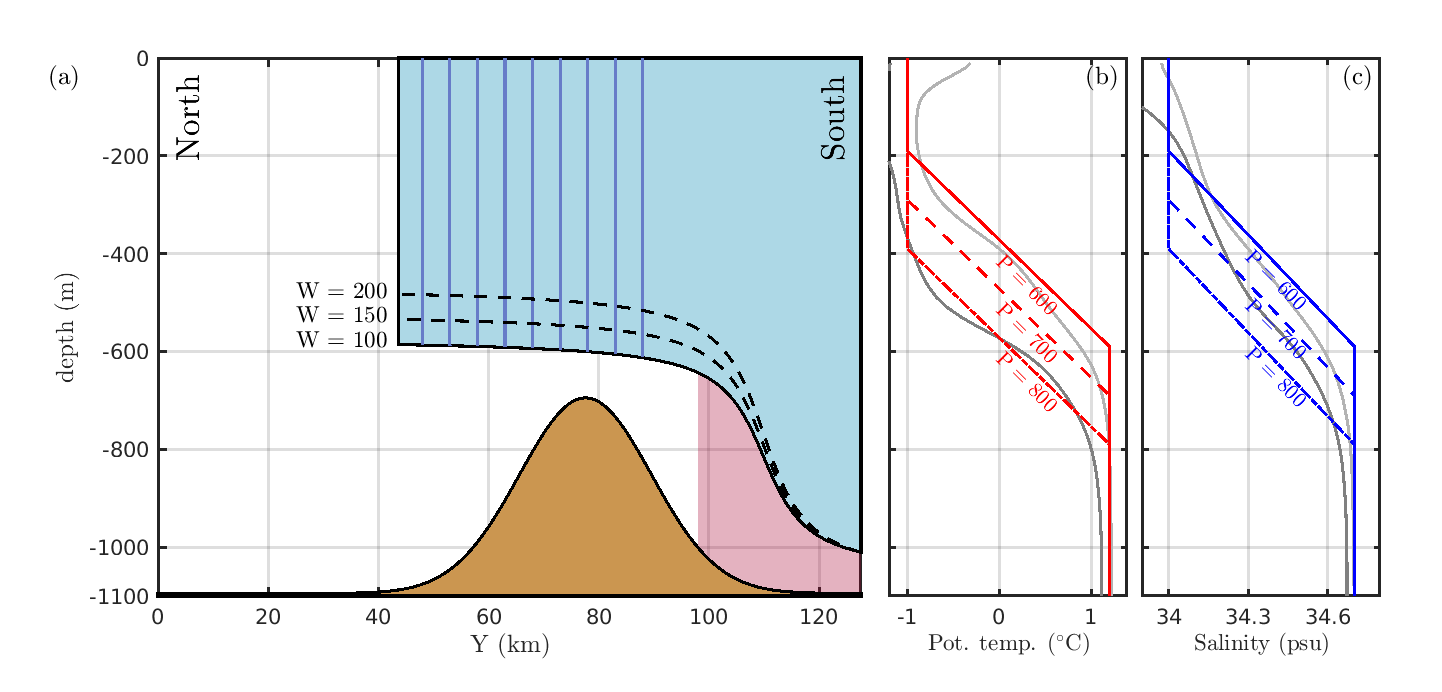
\includegraphics[width = \textwidth]{../make_figures/plots/figure2.eps}
    \caption{(a) Schematic diagram of the experimental setup. The ocean domain consists of the gridded area, which is bordered by a passive ice shelf (shaded blue) and seabed ridge a (shaded brown). Solid and dashed black lines indicate the ice shelf geometry in un-calved case for the three values of the ridge gap parameter $H$ used in the experiments ($H = $100, 200, and 300). Solid blue lines indicate the ice front in the calving experiments, which are located 80, 75, 70, 65, 60, 55, 50, 45, and 40~km north of the southern end of the domain. The red box indicates locations in the ocean domain which are within 30~km of the southern end of the domain, defining the `inner cavity' region, (b) Salinity and temperature profiles used in the experiments (red and blue curves), with $P = 600$ (solid), $P = 700$ (dashed), $P = 800$ (dot-dashed) as indicated by the label. Grey lines correspond to temperature and salinity profiles taken from CTD measurements in Pine Island Bay during the austral summers of 2009 (light grey) and 2012 (dark grey).  \red{Need (a), (b) labels and shade the inner cavity region, change the P800 to dot dashed.} }
    \label{fig:Schematic}
\end{figure}

\subsection{Details of Ocean Model}
The MITgcm is a z-level general circulation model that includes a partial-cell treatment of topography, allowing an accurate description of both the seabed and ice draft. Our model grid consists of 110 layers with a vertical spacing of 10m, and a horizontal resolution of 400m. We use the MITgcm in hydrostatic model with a implicit nonlinear free surface scheme, a third-order direct space-time flux limited advection scheme, a non-linear equation of state~\citeA{Mcdougall2003JAtmosOceanTech}, and the Pacanowski-Philander~\cite{Pacanowski1981JPhysOcean} scheme parametrizes vertical mixing. The equations are solved on an $f$-plane with $f = -1.4\times10^{-4}~\text{s}^{-1}$. \red{maybe say something about viscosity?}

Each simulation is ran for a total of 12 months, using a timestep of 30~\si{seconds}, after which time the configuration reaches a steady state. The melt rates reach approximately 95 percent of their final values with three months (see Appendix). All results presented here are averaged over months nine to twelve in the simulation. 

The MITgcm includes a static representation of ice shelves~\cite{Losch2008JGeophysResOceans}. Ice shelf melting is implemented using the so-called "three-equation formulation"~\cite{Holland1999JPhysOcean} that describes the exchange of heat and salt across the ice-ocean boundary. The implementation of this scheme in MITgcm has been described in detail elsewhere~\cite[for example]{DeRydt2014JGeophysResOceans,Dansereau2014JGROceans} but we note that because the temperatures difference between ice shelves and the adjacent boundary layer is on the order of several degrees Kelvin, thermal exchange across the ice-ocean interface is dominated by latent heat; under this assumption, the three equation formulation gives the melt rate $\dot{m}$ as
\begin{equation}
    \dot{m} = \frac{c_p \gamma_T (T - T_b)}{L}.
\end{equation}
Here $c_p = 3947~\si{\joule \kilogram}^{-1}$, $T$ is the temperature of the ambient ocean, $T_b$ is the temperature, and $\gamma_T$ is a heat exchange co-efficient, which is has an approximately linear relationship on the ocean velocity next to the ice shelf base~\cite{Holland1999JPhysOcean}.

All parameter values used in the three equation formulation here are as in~\citeA{DeRydt2014JGeophysResOceans}, with the exception of the drag co-efficient, which is set to $4.5\times10^{-3}$, a value is more appropriate for Pine Island Glacier~\cite{Dutrieux2014Science} (note, however, that the drag coefficient that enters in the momentum balance, which can be set independently, remains at the default value of $2.5\times 10^{-3}$).

\subsection{Ice Shelf Geometry and Seabed Bathymetry}\label{S:Experiment:Geometry}
Idealized setup is uniform in the zonal direction, with the $x$-axis aligned along the meridional direction and $y$-axis aligned along the zonal direction (we assume that PIG is oriented north-south as is standard, although it's closer to east-west in practice but the beta-effect doesn't make a difference of these scales). Setup shown schematically in figure x. We are primarily interested in understanding how calving changes melt rates in cavities with a topographic barrier to the flow, and our setup includes these features via a seabed ridge and a variable ice shelf front position. 

The sea bed has a Gaussian profile,
\begin{equation}\label{E:Experiment:Bed}
    b(x,y) = 100 \exp\left[-\frac{\left(y - 50\times 10^3\right)^2}{2\sigma^2}\right],
\end{equation}
where $\sigma = 12$~km is the lengthscale over which this profile decays to zero. The profile~\ref{E:Experiment:Bed} corresponds to a ridge of height 400m, which reaches a peak 50km from the southern end of the domain that roughly corresponds to the grounding line (see below). A ridge to grounding line distance of 50km is similar to Pine Island Glacier \red{figure showing PIG bathymetry, slide through ridge and cross section of gaps along ridge}.

In Pine Island, the gap between the ridge and the ice is not constant but varies between ~100m at its narrowest up to greater than 300m at it's widest. This is the result of variability in both the ice shelf draft and the height of the ridge along its length; since we assumed a constant sea bed geometry for simplicity, we aim to capture the effect of this variability by considering values of the gap $H$ between the crest of the seabed ridge and the ice shelf base (see figure). Following~\citeA{DeRydt2014JGeophysResOceans}, we use ice profiles of the form
\begin{equation}
    h(y) = \begin{cases}
    \left(\frac{310 + H}{2.64}\right)\tan^{-1}\left(\frac{y}{5882} -3\right) & \text{for}~y < y_f,\\
    0  & \text{for}~y \geq y_f
    \end{cases}
\end{equation}
where $y_c$ is the location of the ice front (see below). We stress that these ice profiles are not obtained from ice dynamics considerations but feature a flatter section beyond the ridge and a steeper section inside the ridge that is observed in practice \red{figure} (we do not allow the ice profile to reach zero at the southern end of the domain because the MITgcm requires at least two grid cells to permit horizontal exchange of heat and salt) \red{ref?}.

We use three different values of $H$ in different experiment sets. The smallest value we use is $H = 100$m, corresponding to the minimum gap between the ice shelf and ridge that is observed in practice. The largest value of $H$ is  $200$m; as we shall see, the melt response to calving is very small when the cavity gap $H$ is above $200$m, and thus the $H = 200$m case can be thought of an end member for which the cavity does not care about the gap width. The third value of $H$ we use is 150m, which acts as an intermediate value between these two end members.

To simulate calving, we vary the calving front position $y_f$ in each set of experiments; for each set we use ten values in the range $40~\text{km} \leq y_f \leq 84~\text{km}$. The largest value in this range corresponds to the distance of the ice front in PIG in 2012, before significant calving took place in the late 2010s, while the lowest value is determined by a compromise between calving a significant way beyond the ridge, while retaining a significant area that is shared by each experiment, over which the melt rate may be averaged (as we discuss further in \S\ref{S:Baseline}, the area over which melt rates are averaged must be invariant to calving). \red{You might want to but these changes in ice front into the context of PIG, as for hydrography.}


\subsection{Hydrographic Forcing}\label{S:Experiment:Hydrography}

As discussed in \S\ref{S:Introduction}, the presence of a seabed ridge in Pine Island Glacier means that melt rates are particularly sensitive to the hydrographic forcing. It is natural to expect, therefore, that the melting response to calving will also have a sensitive dependence on the hydrographic forcing; to assess the effect of hydrographic forcing on melt response to calving, we repeat each of the sets of `geometric' experiments for three different hydrographic forcings. The hydrographic forcings are imposed on the model by means of a restoring boundary condition at the northern end of the domain: at this restoring boundary, the temperature and salinity are restored to the hydrographic forcings over five grid cells (total length 2km) with a restoring timescale varying from 12~h at the boundary to 60~h at the interior of this restoring regions. (The model includes solid walls with a free slip condition at the southern, western, and eastern sides of the domain.)

%what do our profiles look like
The three hydrographic profiles are shown schematically in figure \red{fig}: both the temperature and salinity vary linearly between constant values in a lower layer (temperature $1.2~\si{\celcius}$, salinity $34.7$~psu) to constant values in an upper layer (temperature $-1~\si{\celcius}$, salinity $34$~psu) across a pyncocline of thickness 400m, which begins at a depth denoted by $P$. The depth $P$ parametrizes the whole profile, with higher $P$ corresponding to a deeper pycnocline; our three hydrographic forcing conditions take $P = 600$, $700$, and $800$. 

%why do we choose these conditions
These piecewise linear hydrographic forcings used in this study correspond to (simplified versions of) typical hydrographic conditions for the Pine Island Bay~\cite{Jacobs1996GRL, Dutrieux2014Science, Jenkins2018NatureGeo} (see figure \red{figure}). The upper and lower layers are dominated by Winter Water and Modified Circumpolar Deep Water, respectively. A record of hydrographic conditions in the Amundsen Sea indicates significant variability in the depth of the pycnocline varies considerably on interannual timescales~\cite{Dutrieux2014Science}; the profiles with $P = 600$ and $P = 800$ correspond to the years 2009 and 2012, respectively, which span the range of observed conditions: in 2012, the average depth of the pycnocline was at the shallowest on record, while in 2009, the average depth of the pycnocline was at the highest on record. As discussed, this resulted in a total yearly freshwater flux that was approximately twice as large in 2009, compared to 2012.

%wrap up the experiments:\ 
Within each experiment set, the "uncalved" geometry, with ice front located 84~km from the southern end of the domain is considered the default. In addition, the experiment set that includes the narrowest gap ($H = 100$) and the highest pycnocline ($P = 600$) is considered the baseline set; in the following section we describe the conditions in the baseline set. \red{maybe better to say (at the start of this section) we have nine experiments, each of which involves resolving the circulation for different calving front positions}

\section{Result for the Baseline Experiments}\label{S:Baseline}
In this section, we describe the results for the baseline experiment with $H = 100$ (the narrowest ridge gap width) and $P = 600$ (the highest pycnocline), corresponding to the solid lines in figure~\ref{fig:Schematic}. We begin by describing the steady state configuration for the uncalved run, and then describe how and why calving changes the inner cavity melt rate.

\subsection{Default Run}
\begin{figure}
    \centering
    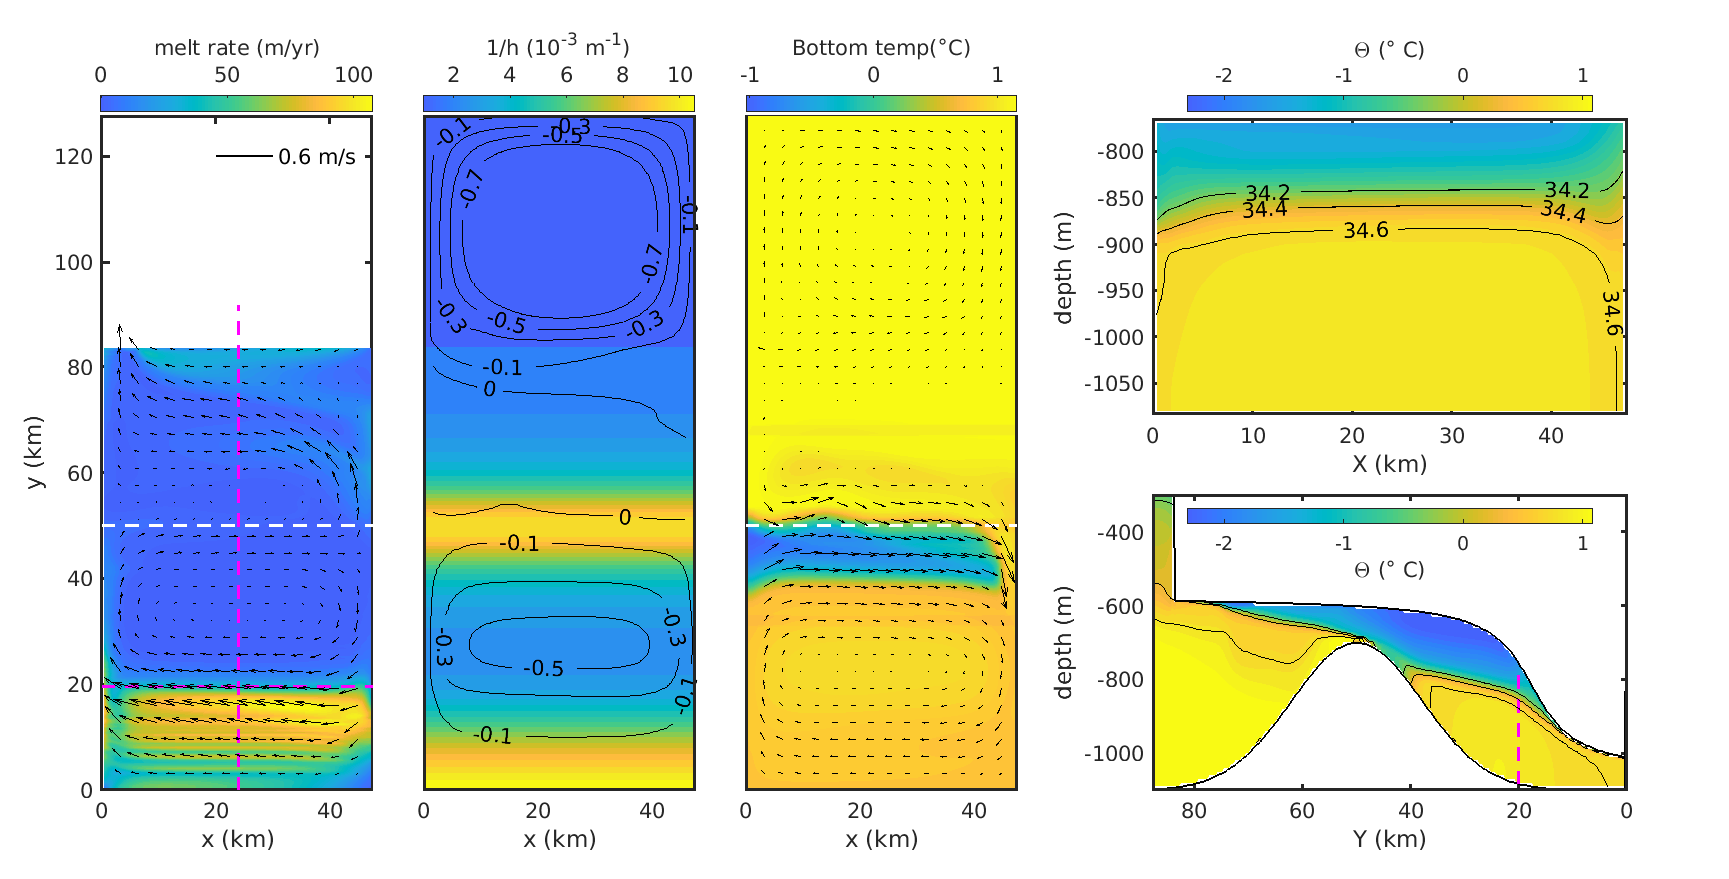
\includegraphics[width = \textwidth]{../make_figures/plots/figure3.eps}
    \caption{(a) Melt rate and BL velocity, (b) BSF and water column thickness, (c) bottom temp and velocity. \red{add a,b,c labels and dashed lines showing the locations of cross sections in figure 6. Also, why not put the colorbars outside?}}
    \label{fig:my_label}
\end{figure}

%figure 4: plots of (a) melt rate and velocity vectors, (b) geostrophic contours and BSF overlain and (c) bottom current and temperature (i.e. a la Jan 2014 paper)
\subsection{Calving effect}
%figure 5: (a) plot of mean melt rate as a function of extent and (b) millgate decomposition 
\begin{figure}
    \centering
    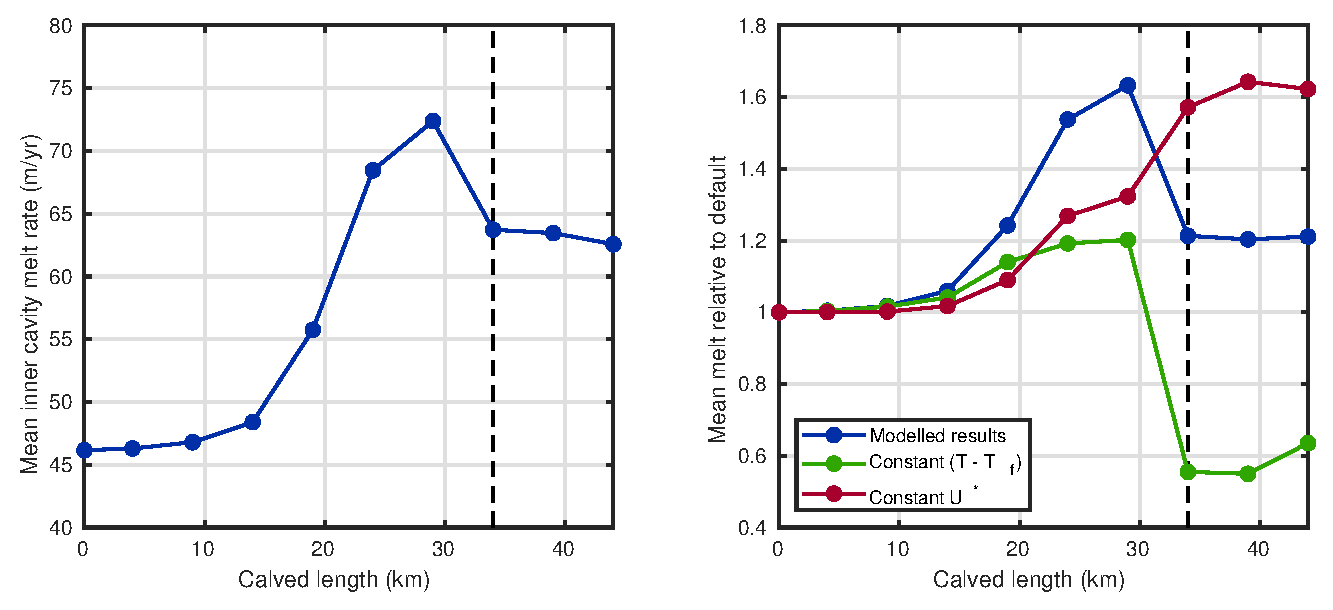
\includegraphics[width = 0.9\textwidth]{../make_figures/plots/figure4.eps}
    \caption{Mean melt rate and velocity/thermal driving decomposition}
    \label{fig:fig4}
\end{figure}

%figure 6: calving with snapping why: (a) row of melt rate (colours) and BSF contours, (b) zonal sections, (c) meridional sections
\begin{figure}
    \centering
    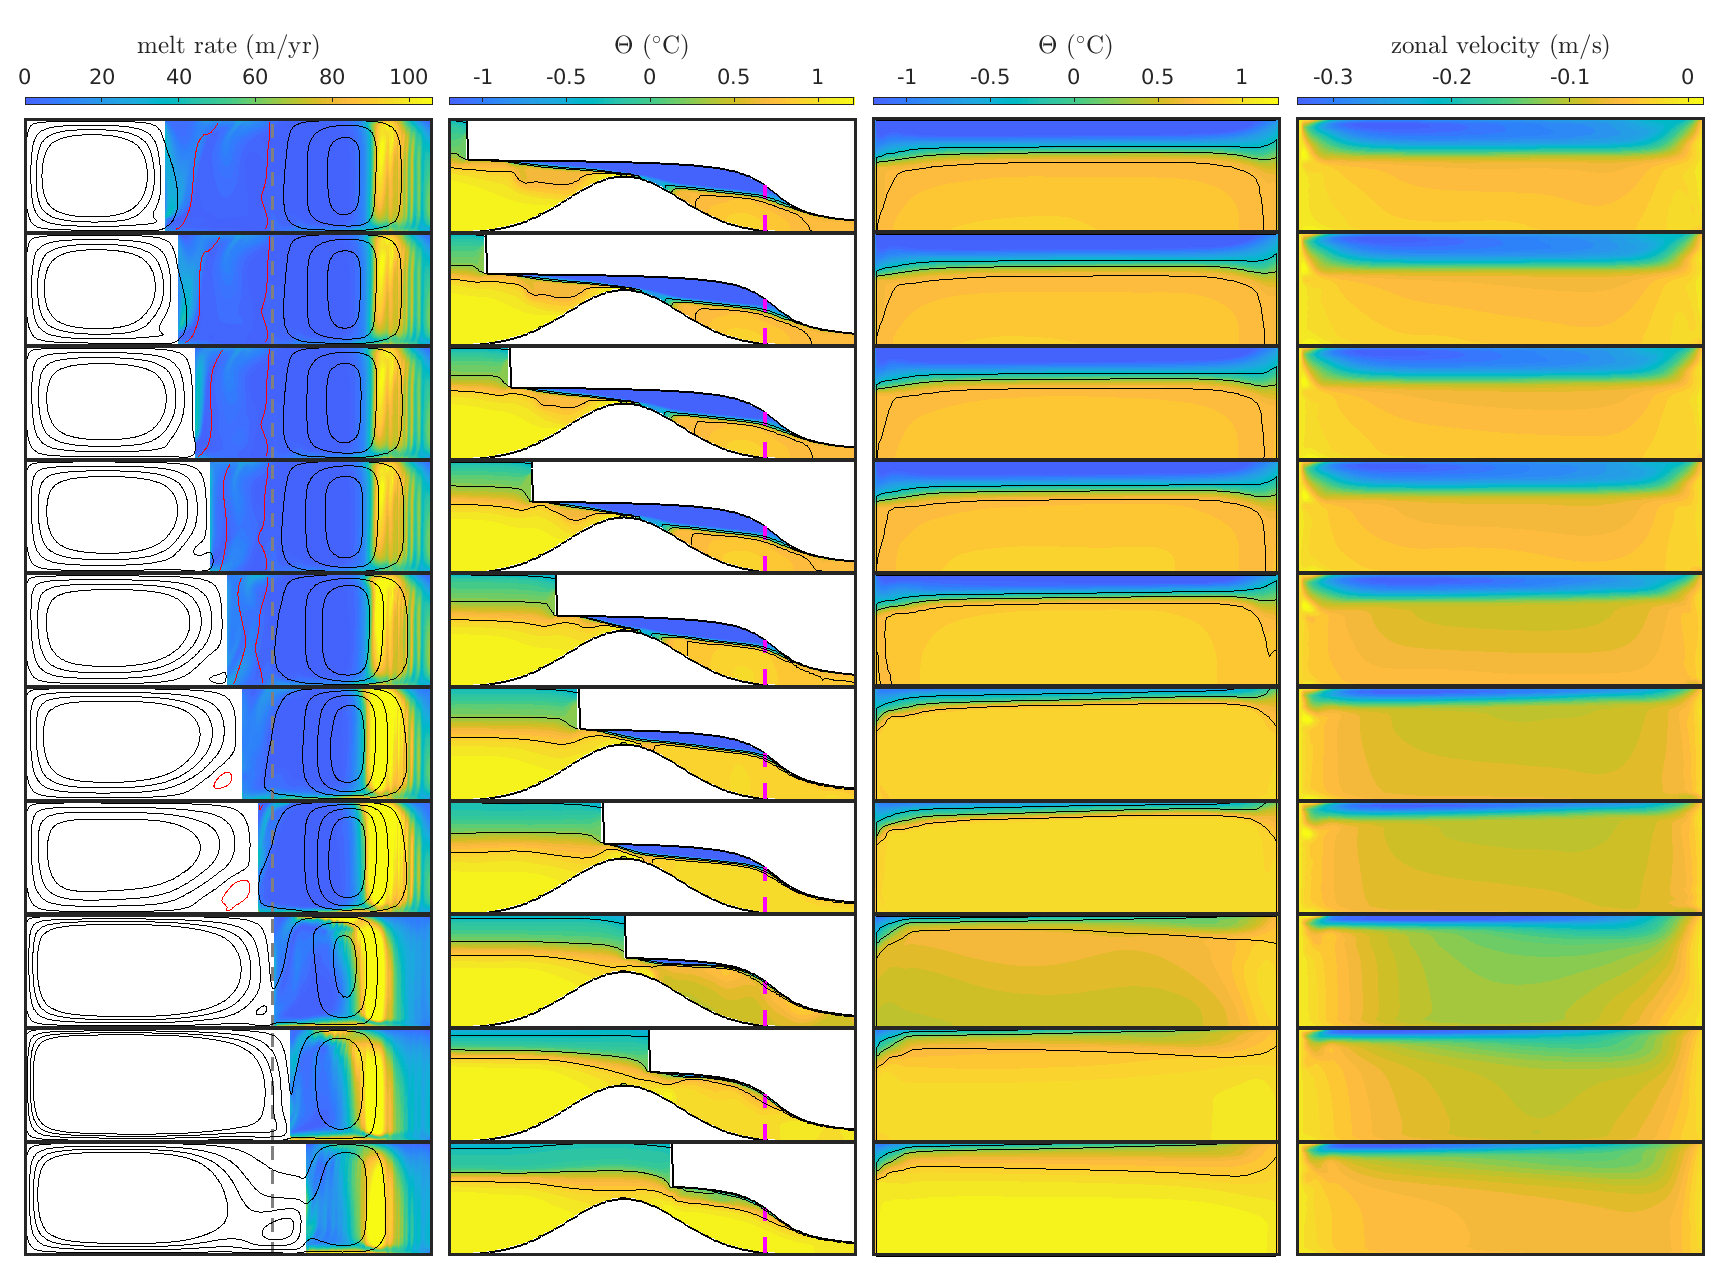
\includegraphics[width = 0.99\textwidth]{../make_figures/plots/figure5.eps}
    \caption{columns showing (a) change of melt rate with snap, (b) meridional cross sectio T and S, (c) zonal cross section T and S, (d) zonal velocity zonal cross section. \red{add a,b,c,d labels for columns and arrow along left with `calving'}}
    \label{fig:fig5}
\end{figure}

\section{Effect of Cavity Geometry on Melt Response to Calving}

\section{Effect of Hydrographic Conditions on Melt Response to Calving}

\section{Discussion}

\section{Summary and Conclusions}




\section{Methods}
To assess the effect of calving events on the sub-shelf melting in Pine Island Glacier, we resolve the cavity circulation an ocean model with a series of sections of the ice shelf removed from a baseline geometry representing the shelf configuration in 2012. We consider a total of 6 different ice shelf geometries (the remaining shelf areas are shown in figure \red{x}): the first two represent realistic situations with ice shelf topography corresponding to 2009 and 2020 and four further simulations in which sections of fast flowing ice are removed. It is important to note that in each simulation, the grounding line position and thickness of the remaining ice shelf are identical to the 2012 conditions; in this way we isolate the effect of a changing shelf front position on melting patterns from other feedback processes [such as?]. \red{define the inner cavity here as the region common to them all, and the reasons why we're interested in this regions: (1) its where the melt is most important and (2) its common to them all, removing the dependence on ice shelf size.}

%ice shelf geometry from Dutrieux 
The sub shelf cavity is computed from the ice and seabed geometry, which we take from~\citeA{Dutrieux2014Science}. Briefly, the ice shelf geometry is calculated from a 40~m-resolution digital elevation model of the ice freeboard from 2008 \red{cite SPIRIT project}, that adjusted using a constant medium bias from observations obtained from the Autosub underwater autonomous vehicle. Note that DEM assumed freely floating ice throughout the shelf, which may reduce its accuracy close to the grounding line. Over the continental shelf, the seabed geometry is well known from ship echo-sounding \red{cite Dutrieux 2014, this sentence is also very similar to their}, while in the cavity it calculated from an inversion of gravimetry data and corrected point-wise using the median difference between the depth from the gravimetry inversion and from the Autosub observations. 

%ocean model details
The ocean model is the MITgcm z-level model (checkpoint 67u) in hydrostatic mode with a grid resolution of 400~m in the horizontal and 10~m in the vertical. The model employs an implicit nonlinear free surface scheme, a third-order direct space-time flux limited advection scheme, a non-linear equation of state~\citeA{Mcdougall2003JAtmosOceanTech}, and the Pacanowski-Philander~\cite{Pacanowski1981JPhysOcean} scheme parametrizes vertical mixing. The equations are solved on an $f$-plane with $f = -1.4\times10^{-4}~\text{s}^{-1}$, which are timestepped using a \red{what scheme?} with a timestep of 30~s. We use constant viscosities of $1~\text{m}^2~\text{s}^{-1}$ and $10^{-5}~\text{m}^2~\text{s}^{-1}$ in the horizontal and vertical, respectively; providing a non-trivial viscosity is necessary for the numerical stability of the model, and we verify that the results presented here are insensitive to the choice of viscosity.

%boundary conditions details (including mention of where they are applied)
As discussed, Pine Island has a strong sensitivity to oceanic conditions and we therefore apply two different sets of forcing conditions corresponding to extrema of observations. At the time, the 2012 conditions were the coldest on record (subsequently overtaken by 2014) and 2009 were the warmest(?) conditions on record [\red{need to mention obs taken at ice shelf front}]. For each of the ice shelf geometries, we perform the simulation with both 2009 and 2012 boundary conditions; that is with ocean temperature and salinity are restored to the corresponding hydrographic observations at the lateral boundaries, giving a total of 12 simulations. In more detail, the model temperature and salinity are relaxed over a weighted mesh of several grid points adjacent to the boundary; we verified that the size this mesh and the timescale over these conditions are applied do not significantly influence the results (\red{Appendix}). Results presented here use a five point mesh whose restoring strength decreases linearly from 100\% at the boundary to 50\% at the fifth grid point away from boundary, and a restoring timescale of one day. \red{Need to mention that ideally we want to model the whole sector but this is impractical so we just use a sector. And we verify that results are insenstiive to the location of the boundary. Probably need to show these profiles in a figure somewhere.}


%ocean ice interaction details
The MITgcm includes a static representation of ice shelves~\cite{Losch2008JGeophysResOceans}, and partial cells with a minimum open-cell fraction of 0.1 are used to better represent the slope ice base. Ice shelf melting is implemented using the so-called "three-equation formulation"~\cite{Holland1999JPhysOcean}, including ice-ocean friction velocity dependent exchange coefficients. We use the standard value of $2.5\times10^{-3}$ for the drag coefficient at the ice-ocean interface that enters into the momentum equations, while the drag coefficient that enters into the three-equation formulation is tuned to $4\times10^{-3}$ to match observations; this choice ensures that the mean of the total meltwater flux for 2009 and 2012 boundary conditions matches the mean of the observed total meltwater flux in 2009 (80 km\textsuperscript{3}/yr) and 2012 (37 km\textsuperscript{3}/yr,~\cite{Dutrieux2014Science}). Note that the model output underestimates the sensitivity to different boundary conditions compared to observations, producing 70 km\textsuperscript{3}/yr and 47 km\textsuperscript{3}/yr for 2009 and 2012 boundary conditions, respectively, but this sensitivity is in line with previous modelling assessments of the sensitivity of Pine Island Glacier to different forcing conditions~\cite{Dutrieux2014Science, DeRydt2014JGeophysResOceans}. \red{Note also that there's a 10\% uncertainty in Dutrieux 2014 observations}

%\begin{itemize}
%    \item To assess the role calving plays in changing melt pattern, we resolve the cavity circulation underneath Pine Island Glacier for a series of different ice shelf geometries (shown in figure). We perform a total of 6 simulations: the first two represent realistic situations with ice shelf topography corresponding to 2012 and 2020 and four further simulations in which sections of fast flowing ice are removed.
%    \item Details of ice shelf topography and verification from Dutrieux 2014, uncertainties discussed in detail there, but we note some of the main ones here. We are not aiming to simulate the ice shelf response to changes in melting, merely to diagnose the magnitude of such changes and it is therefore reasonable to use the same ice geometry with pieces removed.
%    \item As above for bathymetry. Need to plot this, making sure to point out the subglacial ridge.
%    \item Velocities from "Velocity data generated using auto-RIFT (Gardner et al., 2018) and provided by the NASA MEaSUREs ITS\_LIVE project (Gardner et al., 2019)."  (is this the place to mention velocities?) And do you want to show them in plot?

%    \item The cavity circulation is resolved using the MITgcm z-level ocean model in non-hydrostatic mode. Need to include:
 %   \begin{itemize}
  %      \item Checkpoint 67u, 400m resolution in the horizontal, 10m resolution in the vertical. Static representation of ice shelves. Partial cells with a  minimum thickness of 1m allow the bathymetry and ice draft  to be resolved at finer vertical scales. Advection modeled by a 3rd order flux-limited advection scheme. Pacanowski-Philander parametrizes vertical mixing. All runs 1 yr, well beyond steady state being reached. 
   %     \item MITgcm code freely available, driver codes and results processing on github. 
    %    \item \textbf{Do we want to average to total of $\nabla.(h\mathbf{u})$?} Three equation formulation of melting with constant drag coefficient, which is tuned so that the total average of total meltwater flux from fast flowing southern cavity for 2009 (warm) and 2012 (cold) matches the total of $\nabla . (h\mathbf{u})$ using 2012 velocities (approx 50km\textsuperscript{3}/yr), corresponding to an ice shelf that is approximately in balance over the course of a cycle through periodic forcing conditions. Note that our simulations (approx. 70 km\textsuperscript{3}/yr and 50 km\textsuperscript{3}/yr for 2009 and 2012 conditions respectively) underestimate the sensitivity to forcing conditions seen in observations (approx. 80 km\textsuperscript{3}/yr and 37 km\textsuperscript{3}/yr for 2009 and 2012 conditions respectively, but sensitivity is in line with previous simulations reported results (cite Dutrieux). (Need to mention that computed $\nabla . (h\mathbf{u})$ slightly below average of observed 2009 and observed 2012, which is in accordance with a thinning ice shelf)
    %    \item \textbf{or to the observed values?} Three equation formulation of melting with constant drag coefficient, which is tuned to 4$\times$10\textsuperscript{-3} so that the average of total meltwater flux from fast flowing southern cavity for 2009 (warm) and 2012 (cold) matches the same quantity from observations (approx. 80 km\textsuperscript{3}/yr and 37 km\textsuperscript{3}/yr for 2009 and 2012 conditions respectively). Our simulated meltwater fluxes (approx. 70 km\textsuperscript{3}/yr and 50 km\textsuperscript{3}/yr for 2009 and 2012 conditions respectively) have somewhat lower sensitivity to boundary conditions than observations, but note that these sensitivities are in line with previous results (cite Dutrieux). Note that this average (approx 60~km\textsuperscript{3}/yr is larger than the value of obtained by integrating $\nabla.(h\mathbf{u})$ over the shelf (approx 51~km\textsuperscript{3}/yr), which is in accordance with a thinning ice shelf. But note that there's an approx 10\% uncertainty in the observed flux (Dutrieux at al 2014).
      %  \item Note that MITgcm has the option to use different drag coefficient in thermodynamics and momentum equations, and we use the standard value of 2.5$\times$10\textsuperscript{-3} in the momentum equations. Free slip boundary conditions applied on solid boundaries. 
     %   \item Boundary details: apply restoring boundary conditions with timescale on boundary (these are observation as the ice shelf front -- say `following Dutrieux et al 2014'). Model results sensitive to restoring timescale: we use 0.5 day restoring timescale in results presented here, but verify that results similar for different combinations of restoring timescale and drag coefficient which give same total flux when calibrated. We verify that, provided boundary conditions sufficiently far from the shelf front, results are insensitive to boundary location (maybe make the point from Dutrieux 2014 that you really want whole of Amundsen but this is unreasonable). 
    %    \item Sea ice: not sure yet what we want to say about this.
        
    %\end{itemize}

%\end{itemize}

\section{Results}
\begin{figure}
    \centering
    \includegraphics[width = \textwidth]{figs/melt_anomalies_cumulative_2009.eps}
    \caption{Contour plots of (a) the baseline simulated freshwater flux and (b--e) the simulated freshwater flux anomaly (the difference between simulated freshwater flux and the baseline freshwater flux) for different ice shelf scenarios as indicated in each subplot. Each of the simulations presented here uses the 2009 (warm) boundary conditions. The melt rate is ignored in those locations in the shelf which are present before a calving event but not afterwards. The (saturated) colorbar in (b) is appropriate for each of (b)--(e). The corresponding plot using a cumulative measure of the anomaly is presented in the supplementary information. \red{add label of where ridge is, via 750m depth contour?} }
    \label{fig:melt_anomalies_cumulaties_2009}
\end{figure}

The simulated melt rate for the baseline simulation with the 2009 ice shelf geometry and boundary conditions (figure~\ref{fig:melt_anomalies_cumulaties_2009}a) is consistent with observations (figure S\red{x}), with complex features on small scales, but characterized on larger scales as being concentrated near to the grounding line, with a peak melt rate of 120~m~yr\textsuperscript{-1}. \red{describe the current in this scenario}


%going to 2020 gives you a complex change in pattern that is primarily focused at the shelf front
Changing the ice geometry from the 2009 baseline to scenario one (2009 geometry with 2020 ice front) induces a significant, but complex, change in the melt rate pattern, featuring anomalies of up to 50m~yr\textsuperscript{-1} (figure~\ref{fig:melt_anomalies_cumulaties_2009}b). These anomalies are focused at the ice shelf front and are attributed to high velocities associated with upwelling at the new ice shelf front as well as the formation of a gyre in the embayment in the newly open ocean where ice was present in the baseline geometry, but not in 2020 (figure~\ref{fig:barotropic_streamfunction_regular_domain}): this gyre results in a strong circulation along the ice shelf front (the ice shelf front is a dynamic barrier to flow and provides a freshwater source to enhance the flow).
(We verified that this gyre was not related to boundary forcing by repeating the simulations in an extended domain, where the boundary is approximately twice as far from the ice shelf front, and observed little change in the barotropic stream function.) 

The change in geometry from the 2009 baseline to scenario induces only a small change in the melt rates in the inner cavity. This anomaly tends to grow with further sections of ice shelf removal (figure~\ref{fig:melt_anomalies_cumulaties_2009}c--f), particularly close to the northern shear margin, but the pattern is again complex and features locations of significant negative anomalies (indicating melt rates below the 2009 baseline) near to the grounding line. These observations are illustrated further by the plots of mean melt rate and distributions of melt rate anomaly for the inner region in figure~\ref{fig:mean_melt_rate_and_anomaly_distribution}: the mean melt rate increases (the anomalies are enhanced, figure~\ref{fig:mean_melt_rate_and_anomaly_distribution}a), but the distribution of the anomalies becomes wider (the spread of anomalies grows, figure~\ref{fig:mean_melt_rate_and_anomaly_distribution}b) with each further change in geometry. The picture is qualitatively similar for 2012 boundary conditions (figure~\ref{fig:melt_anomalies_2012_cumulative}), although the upper tail on the melt rate anomaly is shorter in this case and the inner cavity anomaly doesn't really appear until scenario 3 (versus scenario 2), but we'll discuss this further later. 

\begin{figure}
    \centering
    \includegraphics[width= \textwidth]{figs/mean_cavity_melt_and_distributions.pdf}
    \caption{Mean melt rate and anomaly distribution. }
    \label{fig:mean_melt_rate_and_anomaly_distribution}
\end{figure}

%why do we get this positive anomaly on average? it seems to be primarily related to heat content (circulation within the cavity is not altered that significantly, but heat content increases significantly with snapping (plot of heat content versus snap), and can see again here that effect focussed on outer shelf after first snap
The increasing average anomaly appears to be primarily the result of heat available for melting in the inner cavity. Although the pattern is again complex, the picture is somewhat clearer than the melt rate: the temperature within the upper boundary layer (computed as the average over the five grid cells nearest to the ice shelf base) increases with further ice shelf removal (figure~\ref{fig:top_temp_anomalies_2009_noncumulative} and figure~\ref{fig:mean_temperature_anomaly}), while the inner cavity velocity does not change significantly -- it is dominated by the aforementioned inner cavity gyre for each of the ice shelf geometries, even those for which the ice shelf front is upstream of the seabed ridge. \red{do you want to be more specific than this? And also mention that you can see the dominating anomaly near the ice shelf front in the mean temperature anomaly plot?}

%how do we quantify the size of the effect? Mean melt rate indicates an approx 10% change in mean melt rate from the first to the last snap. But as discussed, that's skewed by significant positive and negative anomalies and doesn't know anything about geometry. So we came up with this other method.
The average melt rate in the inner cavity can be used as one measure of the importance of the shelf area: for both the 2009 and 2012 boundary conditions, the average melt rate on the inner cavity increases by approximately the same amount after each section of ice shelf is removed ($\approx$ 1m~yr\textsuperscript{-1} and 0.61m~yr\textsuperscript{-1} for 2009 and 2012 boundary condition, respectively), and the mean inner cavity melt rate is approximately 10\% higher in the final scenario than in the baseline. However, this measure is somewhat simplified, and does not capture the broad range of melt rate anomalies (as discussed), as well as not accounting for \emph{where} the melting is applied: \red{sentence explaining why melt anomalies applied in the fast moving regions might be more important? is this even true? Should we sell this metric instead as a measure of the shelf response needed to `fill in' the gap left in shelf stabilization by a change in melt pattern.}. We define a more robust metric that addresses these issues: the `nominal shelf speed-up equivalent', denoted by $\Delta v$, the percentage increase in velocity required to bring the velocity back in line with flux divergence, i.e. $f$ satisfies
    \begin{linenomath*}
    \begin{equation}
    \int_{\text{inner cavity}} \left[\left(1+ \frac{f}{100}\right)\nabla.(h\mathbf{u}) - \dot{m}\right]~\mathbf{d}S = 0.
    \end{equation}
    \end{linenomath*}
    where $h$ and $\mathbf{u}$ are the ice shelf thickness and surface velocity from observations, and $\dot{m}$ is the simulated melt rate.
\red{explain why this known about where the melt is applied (does it?), and explain that this has the added benefit that it phrases the effect in terms of the ice shelf velocity, which is what we are ultimately interested in. Mention straight away that we're not claiming this is the response in velocity we would get, however! Mention that as you increase the velocity, you increase GL flux, but also flux out of this sector? How does this metric tell us about the importance of melt pattern changes -- would be constant if the melt pattern did not change, increases over the baseline can be interpreted how much ice velocity speed up is needed to provide the extra shelf stabilization that is missing because the melt pattern has changed [useful to think in terms of the stabilization of the shelf with snapping as this is how you pitched it earlier].}

%what happens in the baseline case
If the inner cavity  ice flux divergence is completely in balance with melting (i.e. $\mathrm{d}h/\mathrm{d}t = 0)$, then $f = 0$ and no speed up is required to bring the velocity back in line with divergence. \blue{However, it's not quite that simple in the baseline case, because we're using extrema of the periodic cycle.} In the baseline case, the average of the values of $f$ for 2009 and 2012 boundary conditions (i.e. for the average of results corresponding to extrema of the periodic cycle in boundary conditions) is $f \approx 10\%$, which is in agreement with a thinning ice shelf over this period [cite]. We are primarily interested in the \emph{change} in $f$ over this baseline, rather than the actual values. 

%what do we see: for 2009 BC, percentage speedup increases in each subsequent scenario
We see that for the 2009 boundary conditions, the percentage speedup increases with each snap by approximately 3\%. \blue{To put that number in context, the shelf velocity...}. The picture is subtly different for 2012 boundary conditions in two particular ways. Firstly, $f$ does not change when the geometry is changed from the 2009 front to the 2020 front: the change in melt pattern provides no feedback on the inner cavity after this first snap, where as the change is approximately 4\% in the 2012 case. This is attributed to the presence of the ridge: with a low pycnocline, the shelf front position in 2012 is still sufficient to provide a strong barrier to CDW intrusion into the inner cavity, whereas this appears to not be the case for the high pycnocline conditions in 2009. \blue{This can be seen in cross sections? Also motivates further study of how close to the ridge the ice shelf front has to be before you get intrusions}. \red{Can see that the thermocline inside cavity is raised with each snap (see depth $\approx$ 500 -- 700m), until scenario 5 when it drops, but this is in the centre and large melt anomaly persists in the northern shear margin to balance this out -- for 2009 conditions, strong enough to still give an increase in $f$, but for 2012, not strong enough, and $f$ stagnates. This also raises the important point that the largest anomalies are focussed in the shear margins, which are vitally important for stability, but perhaps that belongs in the discussion.}

The second difference is that $f$ is almost for scenario 4 and 5 in the 2012 case (scenario 5 marginally smaller), whereas the latter is larger for the 2009 boundary conditions. This appears to be because the cold anomaly is now able to get over the ridge (can see this in the transects, thermocline on the inner cavity drops after this snap).

%but because of these anomalies of both signs (plot the distribution of melt anomalies, showing large variance?), looking at the mean melt rate anomaly is not necessarily the best measure of size of effect. Also doesn't know anything about \emph{where} the melt is applied. So we come up with this other method...


\section{Discussion and Conclusions}
\begin{itemize}
    \item What do these numbers mean: stress that this is not a prediction for the response to PIG upon calving, which requires a coupled ice ocean model to resolve changes in buttressing etc (this is probably discussion). But this gives us an idea of the magnitude of the changes: difference between melt pattern and no melt pattern increases with snapping and equivalent to (but will not necessarily result in) up to 20\% increase in ice velocity. 
    \item Suggests that melt pattern changes enhance/promote the possibility of a runaway collapse of the shelf.
    \item Some discussion of the location of anomalies: seem to be focused on the shear margins, which is also bad.
    \item What does this mean for melt rate parametrizations?
\end{itemize}

\begin{figure}
    \centering
    \includegraphics[width = \textwidth]{figs/melt_anomalies_cumulative_2012.eps}
    \caption{Cumulative melt anomalies 2012 }
    \label{fig:melt_anomalies_2012_cumulative}
\end{figure}

\begin{figure}
    \centering
    \includegraphics[width = \textwidth]{figs/BSF_2009_extended_domain.eps}
    \caption{Barotropic streamfunction extended domain }
    \label{fig:barotropic_streamfunction_extended_domain}
\end{figure}

\begin{figure}
    \centering
    \includegraphics[width = \textwidth]{figs/BSF_2009_regular_domain.eps}
    \caption{Barotropic streamfunction regular domain }
    \label{fig:barotropic_streamfunction_regular_domain}
\end{figure}

\begin{figure}
    \centering
    \includegraphics[width = \textwidth]{figs/bottom_current_and_temp_2009_cumulative.eps}
    \caption{Bottom temperature and current cumulative with 2009 boundary conditions }
    \label{fig:bottom_temp_anomalies_2009_cumulative}
\end{figure}

\begin{figure}
    \centering
    \includegraphics[width = \textwidth]{figs/bottom_current_and_temp_2012_cumulative.eps}
    \caption{Bottom temperature and current cumulative with 2012 boundary conditions}
    \label{fig:bottom_temp_anomalies_2012_cumulative}
\end{figure}


\begin{figure}
    \centering
    \includegraphics[width = \textwidth]{figs/melt_anomalies_non_cumulative_2009.eps}
    \caption{Melt anomalies 2009 non-cumulative}
    \label{fig:melt_anomalies_2009_noncumulative}
\end{figure}

\begin{figure}
    \centering
    \includegraphics[width = \textwidth]{figs/top_current_and_temp_2009_noncumulative.eps}
    \caption{Temperature anomalies 2009 non-cumulative}
    \label{fig:top_temp_anomalies_2009_noncumulative}
\end{figure}

\begin{figure}
    \centering
    \includegraphics[width = 0.66\textwidth]{figs/mean_temperature_anomaly.eps}
    \caption{Mean top boundary layer temperature anomaly for 2009  (blue) and 2012 (red) boundary conditions. Solid lines correspond to the inner cavity area, which dashed lines correspond to the whole southern ice shelf. }
    \label{fig:mean_temperature_anomaly}
\end{figure}

%%% Suggested section heads:
% \section{Introduction}
%
% The main text should start with an introduction. Except for short
% manuscripts (such as comments and replies), the text should be divided
% into sections, each with its own heading.

% Headings should be sentence fragments and do not begin with a
% lowercase letter or number. Examples of good headings are:

% \section{Materials and Methods}
% Here is text on Materials and Methods.
%
% \subsection{A descriptive heading about methods}
% More about Methods.
%
% \section{Data} (Or section title might be a descriptive heading about data)
%
% \section{Results} (Or section title might be a descriptive heading about the
% results)
%
% \section{Conclusions}


%Text here ===>>>


%%

%  Numbered lines in equations:
%  To add line numbers to lines in equations,
%  \begin{linenomath*}
%  \begin{equation}
%  \end{equation}
%  \end{linenomath*}



%% Enter Figures and Tables near as possible to where they are first mentioned:
%
% DO NOT USE \psfrag or \subfigure commands.
%
% Figure captions go below the figure.
% Table titles go above tables;  other caption information
%  should be placed in last line of the table, using
% \multicolumn2l{$^a$ This is a table note.}
%
%----------------
% EXAMPLE FIGURES
%
% \begin{figure}
% \includegraphics{example.png}
% \caption{caption}
% \end{figure}
%
% Giving latex a width will help it to scale the figure properly. A simple trick is to use \textwidth. Try this if large figures run off the side of the page.
% \begin{figure}
% \noindent\includegraphics[width=\textwidth]{anothersample.png}
%\caption{caption}
%\label{pngfiguresample}
%\end{figure}
%
%
% If you get an error about an unknown bounding box, try specifying the width and height of the figure with the natwidth and natheight options. This is common when trying to add a PDF figure without pdflatex.
% \begin{figure}
% \noindent\includegraphics[natwidth=800px,natheight=600px]{samplefigure.pdf}
%\caption{caption}
%\label{pdffiguresample}
%\end{figure}
%
%
% PDFLatex does not seem to be able to process EPS figures. You may want to try the epstopdf package.
%

%
% ---------------
% EXAMPLE TABLE
%
% \begin{table}
% \caption{Time of the Transition Between Phase 1 and Phase 2$^{a}$}
% \centering
% \begin{tabular}{l c}
% \hline
%  Run  & Time (min)  \\
% \hline
%   $l1$  & 260   \\
%   $l2$  & 300   \\
%   $l3$  & 340   \\
%   $h1$  & 270   \\
%   $h2$  & 250   \\
%   $h3$  & 380   \\
%   $r1$  & 370   \\
%   $r2$  & 390   \\
% \hline
% \multicolumn{2}{l}{$^{a}$Footnote text here.}
% \end{tabular}
% \end{table}

%% SIDEWAYS FIGURE and TABLE
% AGU prefers the use of {sidewaystable} over {landscapetable} as it causes fewer problems.
%
% \begin{sidewaysfigure}
% \includegraphics[width=20pc]{figsamp}
% \caption{caption here}
% \label{newfig}
% \end{sidewaysfigure}
%
%  \begin{sidewaystable}
%  \caption{Caption here}
% \label{tab:signif_gap_clos}
%  \begin{tabular}{ccc}
% one&two&three\\
% four&five&six
%  \end{tabular}
%  \end{sidewaystable}

%% If using numbered lines, please surround equations with \begin{linenomath*}...\end{linenomath*}
%\begin{linenomath*}
%\begin{equation}
%y|{f} \sim g(m, \sigma),
%\end{equation}
%\end{linenomath*}

%%% End of body of article

%%%%%%%%%%%%%%%%%%%%%%%%%%%%%%%%
%% Optional Appendix goes here
%
% The \appendix command resets counters and redefines section heads
%
% After typing \appendix
%
%\section{Here Is Appendix Title}
% will show
% A: Here Is Appendix Title
%
%\appendix
%\section{Here is a sample appendix}

%%%%%%%%%%%%%%%%%%%%%%%%%%%%%%%%%%%%%%%%%%%%%%%%%%%%%%%%%%%%%%%%
%
% Optional Glossary, Notation or Acronym section goes here:
%
%%%%%%%%%%%%%%
% Glossary is only allowed in Reviews of Geophysics
%  \begin{glossary}
%  \term{Term}
%   Term Definition here
%  \term{Term}
%   Term Definition here
%  \term{Term}
%   Term Definition here
%  \end{glossary}

%
%%%%%%%%%%%%%%
% Acronyms
%   \begin{acronyms}
%   \acro{Acronym}
%   Definition here
%   \acro{EMOS}
%   Ensemble model output statistics
%   \acro{ECMWF}
%   Centre for Medium-Range Weather Forecasts
%   \end{acronyms}

%
%%%%%%%%%%%%%%
% Notation
%   \begin{notation}
%   \notation{$a+b$} Notation Definition here
%   \notation{$e=mc^2$}
%   Equation in German-born physicist Albert Einstein's theory of special
%  relativity that showed that the increased relativistic mass ($m$) of a
%  body comes from the energy of motion of the body—that is, its kinetic
%  energy ($E$)—divided by the speed of light squared ($c^2$).
%   \end{notation}




%%%%%%%%%%%%%%%%%%%%%%%%%%%%%%%%%%%%%%%%%%%%%%%%%%%%%%%%%%%%%%%%
%
%  ACKNOWLEDGMENTS
%
% The acknowledgments must list:
%
% >>>>	A statement that indicates to the reader where the data
% 	supporting the conclusions can be obtained (for example, in the
% 	references, tables, supporting information, and other databases).
%
% 	All funding sources related to this work from all authors
%
% 	Any real or perceived financial conflicts of interests for any
%	author
%
% 	Other affiliations for any author that may be perceived as
% 	having a conflict of interest with respect to the results of this
% 	paper.
%
%
% It is also the appropriate place to thank colleagues and other contributors.
% AGU does not normally allow dedications.


\acknowledgments
Enter acknowledgments, including your data availability statement, here.


%% ------------------------------------------------------------------------ %%
%% References and Citations

%%%%%%%%%%%%%%%%%%%%%%%%%%%%%%%%%%%%%%%%%%%%%%%
%
% \bibliography{<name of your .bib file>} don't specify the file extension
%
% don't specify bibliographystyle
%%%%%%%%%%%%%%%%%%%%%%%%%%%%%%%%%%%%%%%%%%%%%%%

\bibliography{mybib}



%Reference citation instructions and examples:
%
% Please use ONLY \cite and \citeA for reference citations.
% \cite for parenthetical references
% ...as shown in recent studies (Simpson et al., 2019)
% \citeA for in-text citations
% ...Simpson et al. (2019) have shown...
%
%
%...as shown by \citeA{jskilby}.
%...as shown by \citeA{lewin76}, \citeA{carson86}, \citeA{bartoldy02}, and \citeA{rinaldi03}.
%...has been shown \cite{jskilbye}.
%...has been shown \cite{lewin76,carson86,bartoldy02,rinaldi03}.
%... \cite <i.e.>[]{lewin76,carson86,bartoldy02,rinaldi03}.
%...has been shown by \cite <e.g.,>[and others]{lewin76}.
%
% apacite uses < > for prenotes and [ ] for postnotes
% DO NOT use other cite commands (e.g., \citet, \citep, \citeyear, \nocite, \citealp, etc.).
%



\end{document}



More Information and Advice:

%% ------------------------------------------------------------------------ %%
%
%  SECTION HEADS
%
%% ------------------------------------------------------------------------ %%

% Capitalize the first letter of each word (except for
% prepositions, conjunctions, and articles that are
% three or fewer letters).

% AGU follows standard outline style; therefore, there cannot be a section 1 without
% a section 2, or a section 2.3.1 without a section 2.3.2.
% Please make sure your section numbers are balanced.
% ---------------
% Level 1 head
%
% Use the \section{} command to identify level 1 heads;
% type the appropriate head wording between the curly
% brackets, as shown below.
%
%An example:
%\section{Level 1 Head: Introduction}
%
% ---------------
% Level 2 head
%
% Use the \subsection{} command to identify level 2 heads.
%An example:
%\subsection{Level 2 Head}
%
% ---------------
% Level 3 head
%
% Use the \subsubsection{} command to identify level 3 heads
%An example:
%\subsubsection{Level 3 Head}
%
%---------------
% Level 4 head
%
% Use the \subsubsubsection{} command to identify level 3 heads
% An example:
%\subsubsubsection{Level 4 Head} An example.
%
%% ------------------------------------------------------------------------ %%
%
%  IN-TEXT LISTS
%
%% ------------------------------------------------------------------------ %%
%
% Do not use bulleted lists; enumerated lists are okay.
% \begin{enumerate}
% \item
% \item
% \item
% \end{enumerate}
%
%% ------------------------------------------------------------------------ %%
%
%  EQUATIONS
%
%% ------------------------------------------------------------------------ %%

% Single-line equations are centered.
% Equation arrays will appear left-aligned.

Math coded inside display math mode \[ ...\]
 will not be numbered, e.g.,:
 \[ x^2=y^2 + z^2\]

 Math coded inside \begin{equation} and \end{equation} will
 be automatically numbered, e.g.,:
 \begin{equation}
 x^2=y^2 + z^2
 \end{equation}


% To create multiline equations, use the
% \begin{eqnarray} and \end{eqnarray} environment
% as demonstrated below.
\begin{eqnarray}
  x_{1} & = & (x - x_{0}) \cos \Theta \nonumber \\
        && + (y - y_{0}) \sin \Theta  \nonumber \\
  y_{1} & = & -(x - x_{0}) \sin \Theta \nonumber \\
        && + (y - y_{0}) \cos \Theta.
\end{eqnarray}

%If you don't want an equation number, use the star form:
%\begin{eqnarray*}...\end{eqnarray*}

% Break each line at a sign of operation
% (+, -, etc.) if possible, with the sign of operation
% on the new line.

% Indent second and subsequent lines to align with
% the first character following the equal sign on the
% first line.

% Use an \hspace{} command to insert horizontal space
% into your equation if necessary. Place an appropriate
% unit of measure between the curly braces, e.g.
% \hspace{1in}; you may have to experiment to achieve
% the correct amount of space.


%% ------------------------------------------------------------------------ %%
%
%  EQUATION NUMBERING: COUNTER
%
%% ------------------------------------------------------------------------ %%

% You may change equation numbering by resetting
% the equation counter or by explicitly numbering
% an equation.

% To explicitly number an equation, type \eqnum{}
% (with the desired number between the brackets)
% after the \begin{equation} or \begin{eqnarray}
% command.  The \eqnum{} command will affect only
% the equation it appears with; LaTeX will number
% any equations appearing later in the manuscript
% according to the equation counter.
%

% If you have a multiline equation that needs only
% one equation number, use a \nonumber command in
% front of the double backslashes (\\) as shown in
% the multiline equation above.

% If you are using line numbers, remember to surround
% equations with \begin{linenomath*}...\end{linenomath*}

%  To add line numbers to lines in equations:
%  \begin{linenomath*}
%  \begin{equation}
%  \end{equation}
%  \end{linenomath*}



